\section{Trích xuất Đặc trưng Thủ công (Handcrafted Features)}
\label{sec:handcrafted_features}

\subsection{Dẫn nhập: Từ "Điểm" đến "Dấu vân tay" Số}
\label{subsec:handcrafted_intro}

Trong các phần trước, chúng ta đã khám phá các thuật toán để phát hiện các \textbf{điểm đặc trưng (keypoints)}—những pixel nổi bật như các góc, vốn có thể được định vị một cách ổn định qua các ảnh khác nhau. Tuy nhiên, việc biết được \textit{vị trí} của một điểm đặc trưng, ví dụ `(x=123, y=456)`, thôi là chưa đủ. Để giải quyết các bài toán phức tạp như nhận dạng vật thể, ghép ảnh panorama, hay tái tạo 3D, chúng ta cần trả lời một câu hỏi sâu hơn: \textit{"Vùng ảnh xung quanh điểm đặc trưng này trông như thế nào?"}

Câu trả lời nằm ở khái niệm \textbf{bộ mô tả đặc trưng (feature descriptor)}. Một bộ mô tả là một vector số, thường có chiều dài cố định, được tính toán từ một vùng ảnh cục bộ (patch) xung quanh một điểm đặc trưng. Nó hoạt động như một "dấu vân tay" số học, chưng cất thông tin về kết cấu (texture), hình dạng (shape), và sự phân bố cường độ sáng của vùng ảnh đó thành một biểu diễn nhỏ gọn, có thể so sánh được về mặt toán học.

Một bộ mô tả lý tưởng cần cân bằng một cách tinh tế giữa hai thuộc tính có phần đối lập nhau:

\begin{enumerate}
    \item \textbf{Tính Phân biệt (Distinctiveness):} Các vùng ảnh khác nhau về mặt cấu trúc (ví dụ: một vùng chứa góc của một con mắt và một vùng chứa góc của một tòa nhà) phải tạo ra các vector mô tả khác xa nhau trong không gian đặc trưng. Khoảng cách Euclid (hoặc một thước đo phù hợp khác) giữa các vector này phải lớn. Điều này cho phép chúng ta phân biệt giữa các đối tượng và các phần khác nhau của cùng một đối tượng.

    \item \textbf{Tính Bất biến (Invariance):} Các vùng ảnh giống nhau về mặt ngữ nghĩa (ví dụ: cùng một góc của tòa nhà), nhưng được chụp dưới các điều kiện khác nhau, phải tạo ra các vector mô tả gần giống nhau. Đây là thuộc tính quan trọng nhất, cho phép chúng ta "nhận ra" cùng một thứ dù góc nhìn thay đổi. Các loại bất biến chính bao gồm:
    \begin{itemize}
        \item \textbf{Bất biến Hình học (Geometric Invariance):}
            \begin{itemize}
                \item \textit{Bất biến với Tịnh tiến (Translation):} Được đảm bảo vì bộ mô tả được tính toán cục bộ xung quanh điểm đặc trưng.
                \item \textit{Bất biến với Xoay (Rotation):} Đặc trưng không thay đổi khi ảnh bị xoay.
                \item \textit{Bất biến với Tỷ lệ (Scale):} Đặc trưng không thay đổi khi đối tượng được phóng to hoặc thu nhỏ.
                \item \textit{Bất biến Affine (Affine Invariance):} Đặc trưng không thay đổi dưới các phép biến đổi affine (xoay, tỷ lệ, cắt xiên), vốn là một xấp xỉ tốt cho sự thay đổi góc nhìn 3D khi nhìn từ xa.
            \end{itemize}
        \item \textbf{Bất biến Quang học (Photometric Invariance):}
            \begin{itemize}
                \item \textit{Bất biến với Độ sáng (Illumination):} Đặc trưng không thay đổi khi độ sáng chung của ảnh tăng hoặc giảm.
                \item \textit{Bất biến với Độ tương phản (Contrast):} Đặc trưng không thay đổi khi độ tương phản của ảnh thay đổi.
            \end{itemize}
    \end{itemize}
\end{enumerate}

Kỷ nguyên Thị giác Máy tính cổ điển là một cuộc chạy đua trong việc thiết kế các bộ mô tả thủ công ngày càng mạnh mẽ, với mục tiêu cân bằng giữa tính phân biệt, tính bất biến, và hiệu suất tính toán. Trong phần này, chúng ta sẽ đi sâu vào bốn trong số những bộ mô tả có ảnh hưởng nhất trong lịch sử: SIFT, SURF, ORB, và HOG. Hiểu được chúng không chỉ giúp chúng ta nắm vững các kỹ thuật nền tảng mà còn cung cấp một trực giác sâu sắc về bản chất của việc "học biểu diễn" (representation learning) mà các mạng nơ-ron hiện đại đang cố gắng tự động hóa.

\subsection{SIFT (Scale-Invariant Feature Transform)}
\label{subsec:sift}

Được giới thiệu bởi David Lowe vào năm 2004 \cite{Lowe2004}, \textbf{Scale-Invariant Feature Transform (SIFT)} là một cột mốc vĩ đại, được cho là một trong những thuật toán quan trọng và có ảnh hưởng nhất trong lịch sử Thị giác Máy tính. SIFT không chỉ là một bộ mô tả; nó là một pipeline hoàn chỉnh bao gồm cả việc phát hiện điểm đặc trưng và mô tả chúng. Sức mạnh phi thường của nó nằm ở khả năng tạo ra các đặc trưng có tính \textbf{bất biến cao với sự thay đổi về tỷ lệ (scale), xoay (rotation), và một phần thay đổi về ánh sáng và góc nhìn 3D}.

Quy trình của SIFT bao gồm bốn bước chính, mỗi bước được thiết kế tỉ mỉ để giải quyết một loại bất biến cụ thể.

\subsubsection{Bước 1: Phát hiện Điểm cực trị trong Không gian Tỷ lệ (Scale-Space Extrema Detection)}
\label{subsubsec:sift_scale_space}
\textbf{Mục tiêu:} Đạt được tính bất biến với tỷ lệ.
\textbf{Trực giác:} Một đối tượng chỉ có "ý nghĩa" ở một tỷ lệ nhất định. Một góc của tòa nhà có thể là một đặc trưng tốt ở một khoảng cách nhất định, nhưng khi bạn zoom lại rất gần, nó chỉ là một đường thẳng. Để tìm các đặc trưng ổn định, chúng ta phải tìm chúng ở "tỷ lệ đặc trưng" của chúng. SIFT thực hiện điều này bằng cách tìm kiếm trên một cấu trúc đa tỷ lệ gọi là \textbf{không gian tỷ lệ (scale-space)}.

\begin{enumerate}
    \item \textbf{Xây dựng Kim tự tháp Gaussian (Gaussian Pyramid):} Ảnh gốc $I(x, y)$ được làm mờ liên tục bằng các bộ lọc Gaussian $G(x, y, \sigma)$ với giá trị độ lệch chuẩn $\sigma$ tăng dần.
    \begin{equation}
        L(x, y, \sigma) = G(x, y, \sigma) * I(x, y)
    \end{equation}
    Sau mỗi một số lần làm mờ (một \textit{octave}), ảnh được giảm một nửa kích thước (downsample) và quá trình làm mờ được lặp lại. Kết quả là một tập hợp các ảnh được làm mờ ở nhiều mức độ và nhiều kích thước khác nhau, tạo thành một kim tự tháp. Mỗi "tầng" của kim tự tháp được gọi là một octave.

    \item \textbf{Xây dựng Kim tự tháp Hiệu của Gaussian (Difference-of-Gaussian - DoG):} Thay vì sử dụng trực tiếp các ảnh Gaussian, SIFT tính toán hiệu số giữa các cặp ảnh Gaussian kề nhau trong cùng một octave.
    \begin{equation}
        D(x, y, \sigma) = L(x, y, k\sigma) - L(x, y, \sigma)
        \label{eq:sift_dog}
    \end{equation}
    trong đó $k$ là một hằng số.

    \begin{mdframed}[style=infobox]
    \textbf{Trực giác Toán học: Tại sao dùng DoG?}
    
    Hàm DoG là một phép xấp xỉ hiệu quả về mặt tính toán của hàm \textbf{Laplacian của Gaussian chuẩn hóa theo tỷ lệ (scale-normalized Laplacian of Gaussian - $\sigma^2 \nabla^2 G$)}. Hàm LoG là một bộ phát hiện "đốm" (blob detector) rất tốt, vì toán tử Laplacian ($\nabla^2$) đo lường "độ cong" hoặc "sự lồi lõm" của hàm cường độ ảnh. Một điểm cực trị của hàm LoG tương ứng với tâm của một vùng sáng trên nền tối hoặc ngược lại.
    
    Theo lý thuyết không gian tỷ lệ, có thể chứng minh rằng:
    \begin{equation}
        \frac{\partial G}{\partial \sigma} = \sigma \nabla^2 G
    \end{equation}
    Sử dụng định nghĩa đạo hàm bằng sai phân hữu hạn, ta có:
    \begin{equation}
        \sigma \nabla^2 G \approx \frac{G(x, y, k\sigma) - G(x, y, \sigma)}{k\sigma - \sigma}
    \end{equation}
    Do đó, $G(k\sigma) - G(\sigma) \approx (k-1)\sigma^2 \nabla^2 G$. Điều này cho thấy $D(x,y,\sigma)$ trong công thức \ref{eq:sift_dog} tỷ lệ với LoG chuẩn hóa theo tỷ lệ. Việc trừ hai ảnh Gaussian đã được làm mờ sẵn nhanh hơn rất nhiều so với việc tính toán đạo hàm bậc hai một cách tường minh.
    \end{mdframed}

    \item \textbf{Tìm các Điểm cực trị cục bộ:} Một pixel được chọn làm ứng cử viên điểm đặc trưng nếu giá trị của nó trong kim tự tháp DoG là một cực đại hoặc cực tiểu cục bộ so với 26 lân cận của nó: 8 lân cận trong cùng ảnh DoG, 9 lân cận trong ảnh DoG ở tỷ lệ trên, và 9 lân cận trong ảnh DoG ở tỷ lệ dưới.
\end{enumerate}

\begin{center}
    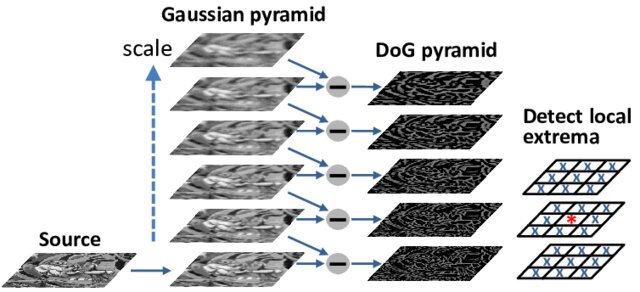
\includegraphics[width=1.0\textwidth]{images/sift_dog_pyramid.jpg}
    \captionof{figure}{Quy trình phát hiện điểm đặc trưng trong SIFT. (Trái) Ảnh gốc được làm mờ liên tục để tạo các octave của kim tự tháp Gaussian. (Giữa) Các ảnh Gaussian kề nhau được trừ đi để tạo kim tự tháp Hiệu của Gaussian (DoG). (Phải) Các điểm cực trị (đánh dấu X) được tìm thấy bằng cách so sánh một pixel với 26 lân cận của nó trong không gian 3D (không gian 2D và chiều tỷ lệ).}
    \label{fig:sift_dog_pyramid}
\end{center}

\subsubsection{Bước 2: Định vị chính xác Điểm đặc trưng và Lọc bỏ (Accurate Keypoint Localization)}
\label{subsubsec:sift_localization}
Các điểm cực trị tìm thấy ở bước 1 chỉ là các ứng cử viên và vị trí của chúng là rời rạc. Bước này thực hiện tinh lọc để tăng độ chính xác và độ ổn định.

\begin{enumerate}
    \item \textbf{Nội suy vị trí chính xác:} Một mô hình Taylor bậc hai được khớp vào vùng lân cận của điểm ứng cử viên trong không gian 3D (x, y, $\sigma$) để nội suy vị trí chính xác của điểm cực trị với độ chính xác dưới pixel (sub-pixel) và dưới tỷ lệ (sub-scale). Vị trí của điểm cực trị $\hat{\mathbf{x}}$ được tìm bằng cách giải phương trình đạo hàm bậc nhất bằng 0:
    \begin{equation}
        \hat{\mathbf{x}} = - \frac{\partial^2 D^{-1}}{\partial \mathbf{x}^2} \frac{\partial D}{\partial \mathbf{x}}
    \end{equation}
    
    \item \textbf{Loại bỏ các điểm có độ tương phản thấp:} Giá trị của hàm DoG tại vị trí cực trị nội suy, $|D(\hat{\mathbf{x}})|$, được so sánh với một ngưỡng (ví dụ: 0.03). Nếu giá trị này quá nhỏ, điểm đặc trưng được coi là không ổn định và nhạy cảm với nhiễu, do đó sẽ bị loại bỏ.

    \item \textbf{Loại bỏ các phản ứng trên cạnh (Edge response):} Các điểm cực trị DoG có xu hướng phản ứng mạnh dọc theo các cạnh, vốn là những đặc trưng không được định vị tốt. Để loại bỏ chúng, SIFT sử dụng ma trận Hessian $2 \times 2$ tại điểm đặc trưng:
    \begin{equation}
        \mathbf{H} = \begin{bmatrix} D_{xx} & D_{xy} \\ D_{xy} & D_{yy} \end{bmatrix}
    \end{equation}
    Các trị riêng của $\mathbf{H}$ ($\alpha$ và $\beta$) tỷ lệ với độ cong chính của hàm $D$. Đối với một cạnh, sẽ có một độ cong lớn theo hướng vuông góc với cạnh và độ cong nhỏ theo hướng song song với cạnh, dẫn đến một trị riêng lớn và một trị riêng nhỏ. SIFT sử dụng tỷ lệ giữa các trị riêng này để loại bỏ các điểm giống cạnh. Thay vì tính toán trực tiếp các trị riêng, một phương pháp hiệu quả hơn được sử dụng, dựa trên Dấu vết (Trace) và Định thức (Determinant) của Hessian:
    \begin{equation}
        \frac{\text{Tr}(\mathbf{H})^2}{\text{Det}(\mathbf{H})} = \frac{(D_{xx} + D_{yy})^2}{D_{xx}D_{yy} - D_{xy}^2} = \frac{(\alpha + \beta)^2}{\alpha \beta} = \frac{(r+1)^2}{r}
    \end{equation}
    với $r = \alpha/\beta$. Nếu tỷ lệ này lớn hơn một ngưỡng (ví dụ: 10), điểm đặc trưng được coi là nằm trên một cạnh và bị loại bỏ.
\end{enumerate}

\subsubsection{Bước 3: Gán Hướng (Orientation Assignment)}
\label{subsubsec:sift_orientation}
\textbf{Mục tiêu:} Đạt được tính bất biến với xoay.
\textbf{Trực giác:} Bằng cách xác định một hướng "chuẩn" cho mỗi điểm đặc trưng, chúng ta có thể xoay vùng ảnh cục bộ về hướng chuẩn đó trước khi tính toán bộ mô tả. Điều này đảm bảo rằng dù ảnh gốc bị xoay như thế nào, vùng ảnh dùng để tính toán bộ mô tả luôn có cùng một hướng.

\begin{enumerate}
    \item Đối với mỗi điểm đặc trưng, một vùng lân cận xung quanh nó (có bán kính phụ thuộc vào tỷ lệ $\sigma$ của điểm đặc trưng) được xem xét.
    \item Tại mỗi pixel trong vùng lân cận, độ lớn $m(x,y)$ và hướng $\theta(x,y)$ của gradient được tính toán.
    \item Một biểu đồ hướng (orientation histogram) gồm 36 bin (mỗi bin 10 độ) được tạo ra. Mỗi pixel trong vùng lân cận sẽ "bỏ phiếu" vào một bin tương ứng với hướng của nó. Trọng số của mỗi phiếu bầu là độ lớn gradient $m(x,y)$ của pixel đó, được nhân với một trọng số Gaussian để giảm ảnh hưởng của các pixel ở xa tâm.
    \item Các đỉnh cao nhất trong biểu đồ được xác định. Hướng của đỉnh cao nhất được gán làm hướng chính. Bất kỳ đỉnh nào khác có độ cao trong vòng 80\% của đỉnh cao nhất cũng được giữ lại, và một điểm đặc trưng mới sẽ được tạo ra cho mỗi hướng đó (có cùng vị trí và tỷ lệ nhưng khác hướng). Điều này giúp SIFT xử lý tốt các vùng có cấu trúc đối xứng.
\end{enumerate}

\subsubsection{Bước 4: Tạo Bộ mô tả Đặc trưng (Descriptor Generation)}
\label{subsubsec:sift_descriptor}
Đây là bước cuối cùng, tạo ra "dấu vân tay" 128 chiều.
\begin{enumerate}
    \item Lấy một vùng lân cận $16 \times 16$ pixel xung quanh điểm đặc trưng.
    \item \textbf{Xoay vùng lân cận này theo hướng chính} đã được xác định ở bước 3. Điều này đảm bảo bộ mô tả sẽ có \textbf{tính bất biến với xoay}. Các giá trị pixel tại các tọa độ mới được nội suy song tuyến tính.
    \item Chia vùng $16 \times 16$ này thành một lưới $4 \times 4$ các ô, mỗi ô có kích thước $4 \times 4$ pixel. Việc chia nhỏ này giúp bộ mô tả có khả năng chịu được các biến dạng hình học nhỏ.
    \item Trong mỗi ô $4 \times 4$, tính toán một biểu đồ hướng gradient gồm 8 bin. Tương tự như bước 3, mỗi pixel trong ô sẽ bỏ phiếu vào biểu đồ này với trọng số là độ lớn gradient của nó. Hướng gradient được tính tương đối so với hướng chính của điểm đặc trưng.
    \item Nối (concatenate) tất cả 16 biểu đồ (mỗi biểu đồ 8 giá trị) lại với nhau để tạo thành một vector đặc trưng duy nhất có $16 \text{ ô} \times 8 \text{ bin/ô} = 128$ chiều.
    \item \textbf{Chuẩn hóa vector 128 chiều này về độ dài đơn vị (norm L2).} Bước này cực kỳ quan trọng để đạt được \textbf{tính bất biến với sự thay đổi độ sáng tuyến tính}. Ví dụ, tăng độ sáng toàn bộ ảnh lên gấp đôi sẽ làm tăng độ lớn của tất cả các gradient lên gấp đôi, nhưng sau khi chuẩn hóa L2, vector kết quả sẽ không đổi.
    \item Sau khi chuẩn hóa, các giá trị trong vector lớn hơn một ngưỡng (thường là 0.2) sẽ bị cắt bớt (clipped) về 0.2, và vector được chuẩn hóa lại. Bước này giúp giảm ảnh hưởng của các thay đổi ánh sáng phi tuyến, ví dụ như sự bão hòa của cảm biến máy ảnh.
\end{enumerate}

\begin{center}
    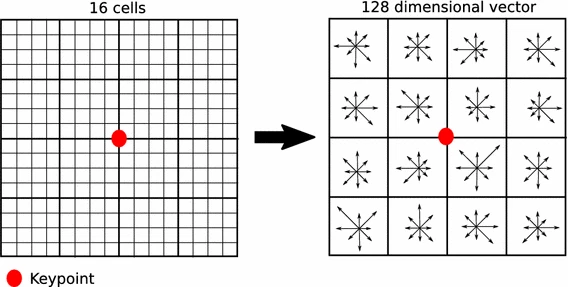
\includegraphics[width=0.9\textwidth]{images/sift_descriptor_generation.png}
    \captionof{figure}{Quy trình tạo bộ mô tả SIFT. (1) Một vùng lân cận $16 \times 16$ được lấy xung quanh điểm đặc trưng và được xoay theo hướng chính. (2) Vùng này được chia thành lưới $4 \times 4$. (3) Trong mỗi ô $4 \times 4$, một biểu đồ hướng 8-bin được tính toán. (4) Tất cả 16 biểu đồ được nối lại tạo thành một vector 128 chiều, sau đó được chuẩn hóa.}
    \label{fig:sift_descriptor}
\end{center}

Kết quả là một vector 128-D cực kỳ mạnh mẽ, đã đặt ra tiêu chuẩn vàng cho việc so khớp đặc trưng trong nhiều năm. Tuy nhiên, sự phức tạp của nó cũng là điểm yếu: SIFT khá chậm về mặt tính toán cho các ứng dụng thời gian thực.

\subsection{SURF (Speeded-Up Robust Features)}
\label{subsec:surf}

Được giới thiệu bởi Herbert Bay và các đồng nghiệp vào năm 2006 \cite{Bay2006}, \textbf{SURF} được thiết kế như một phiên bản \textit{nhanh hơn} của SIFT, trong khi vẫn duy trì (và đôi khi vượt qua) độ mạnh mẽ của nó đối với thay đổi tỷ lệ, góc quay và ánh sáng. SURF đạt được tốc độ cao hơn nhờ việc sử dụng các phép tính xấp xỉ thông minh, đặc biệt là dựa trên \textbf{ảnh tích phân (integral images)} và \textbf{bộ lọc hộp (box filters)} để mô phỏng các đạo hàm Gaussian một cách hiệu quả.

Khác với SIFT, SURF được tối ưu hóa để thực hiện trong thời gian thực và dễ dàng triển khai trên phần cứng có khả năng song song (như GPU hoặc FPGA).

\subsubsection{Phát hiện Điểm đặc trưng: Xấp xỉ Hessian bằng Box Filter và Integral Image}
\label{subsubsec:surf_detection}

\begin{enumerate}
	\item \textbf{Ảnh Tích phân (Integral Image):}  
	Đây là nền tảng giúp SURF đạt được tốc độ vượt trội. Một ảnh tích phân $I_{ii}$ tại vị trí $(x, y)$ được định nghĩa là tổng của tất cả các giá trị pixel nằm ở phía trên và bên trái của điểm đó, bao gồm cả chính nó:
	\begin{equation}
		I_{ii}(x, y) = \sum_{i=0}^{x} \sum_{j=0}^{y} I(i, j)
	\end{equation}
	Nhờ đặc tính cộng dồn, tổng giá trị của các pixel trong \textit{bất kỳ vùng chữ nhật nào} có thể được tính cực nhanh chỉ bằng 4 phép truy cập bộ nhớ và 3 phép cộng/trừ, bất kể kích thước của vùng đó.  
	Điều này cho phép các phép tích chập với các bộ lọc hộp được thực hiện tức thời mà không cần duyệt qua từng pixel.
	
	\item \textbf{Xấp xỉ Hessian bằng Bộ lọc hộp (Box Filters):}  
	SURF sử dụng ma trận Hessian để phát hiện các vùng có độ biến thiên cường độ mạnh (tương ứng với các điểm đặc trưng). Tuy nhiên, thay vì tính toán đạo hàm Gaussian chính xác như SIFT, SURF \textit{xấp xỉ} các đạo hàm bậc hai ($D_{xx}, D_{yy}, D_{xy}$) bằng các \textbf{bộ lọc hộp} kích thước khác nhau.  
	Nhờ ảnh tích phân, việc áp dụng các bộ lọc này có độ phức tạp tính toán hằng số ($O(1)$).  
	Determinant của Hessian xấp xỉ được tính như sau:
	\begin{equation}
		\text{Det}(\mathbf{H}_{\text{approx}}) = D_{xx}D_{yy} - (w D_{xy})^2
	\end{equation}
	trong đó $w$ là trọng số hiệu chỉnh (thường $w = 0.9$) để cân bằng ảnh hưởng của các đạo hàm chéo.
	
	\item \textbf{Xây dựng Không gian Tỷ lệ:}  
	Không giống như SIFT (giảm kích thước ảnh và giữ nguyên bộ lọc), SURF làm ngược lại: \textbf{giữ nguyên ảnh gốc và mở rộng kích thước bộ lọc hộp}.  
	Cách tiếp cận này có hai ưu điểm:  
	(1) Tránh mất mát thông tin do nội suy hoặc giảm mẫu ảnh;  
	(2) Tận dụng tốt hơn khả năng song song, vì mọi phép tính được thực hiện trên cùng độ phân giải.
\end{enumerate}

\begin{center}
	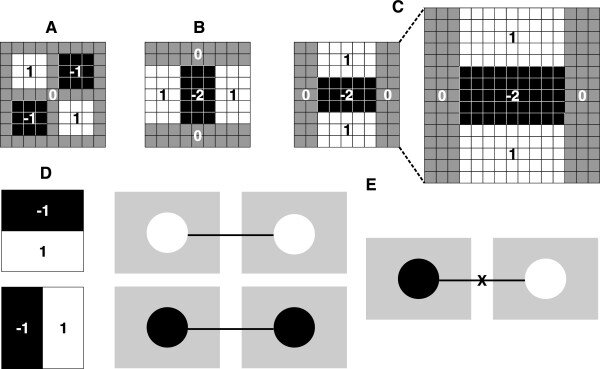
\includegraphics[width=0.9\textwidth]{images/surf_box_filters.jpg}
	\captionof{figure}{Xấp xỉ đạo hàm bậc hai trong SURF. (Trái) Các bộ lọc hộp mô phỏng $D_{yy}$ (trên) và $D_{xy}$ (dưới). Vùng xám biểu thị trọng số âm, vùng trắng biểu thị trọng số dương. (Phải) Nhờ ảnh tích phân, tổng giá trị pixel trong mỗi vùng được tính nhanh chóng mà không cần duyệt từng điểm ảnh.}
	\label{fig:surf_box_filters}
\end{center}

Sau khi tính toán, các \textbf{điểm đặc trưng} được chọn là các cực đại cục bộ của giá trị determinant Hessian trong cả không gian và tỷ lệ (so sánh trong lân cận $3 \times 3 \times 3$).

\subsubsection{Gán Hướng và Tạo Bộ mô tả}
\label{subsubsec:surf_descriptor}
\begin{enumerate}
	\item \textbf{Gán Hướng:}  
	SURF sử dụng các \textbf{đáp ứng Haar wavelet} theo hai hướng $x$ và $y$ trong vùng lân cận hình tròn bán kính $6\sigma$ quanh điểm đặc trưng.  
	Các đáp ứng này được nhân trọng số Gaussian để giảm nhiễu, rồi cộng gộp trong các cung 60° để tìm hướng chính có năng lượng mạnh nhất.  
	Cách tiếp cận này đơn giản hơn nhiều so với biểu đồ hướng của SIFT, nhưng vẫn đảm bảo tính bất biến góc quay.
	
	\item \textbf{Tạo Bộ mô tả (Descriptor Construction):}
	\begin{itemize}
		\item Chọn vùng $20\sigma \times 20\sigma$ quanh điểm đặc trưng và xoay theo hướng chính tìm được ở bước trước.  
		\item Chia vùng này thành lưới $4 \times 4$ các ô con (subregion).  
		\item Trong mỗi ô con, tính toán các đáp ứng Haar wavelet theo $x$ ($dx$) và $y$ ($dy$) tại các điểm mẫu $5 \times 5$.  
		\item Mỗi ô con tạo ra một vector 4 chiều:
		\[
		\mathbf{v} = (\sum dx, \sum |dx|, \sum dy, \sum |dy|)
		\]
		\item Ghép 16 vector này lại với nhau, ta thu được bộ mô tả 64 chiều. Phiên bản mở rộng (\textbf{SURF-128}) tăng khả năng phân biệt bằng cách tách riêng các tổng dương và âm của $dx, dy$.
	\end{itemize}
\end{enumerate}

\paragraph{Đánh giá tổng quan:}  
SURF là một ví dụ điển hình về việc \textbf{tối ưu hóa tốc độ mà vẫn duy trì độ ổn định}.  
Nó đánh đổi độ chính xác của phép xấp xỉ Gaussian để đổi lấy tốc độ xử lý tăng gấp nhiều lần nhờ ảnh tích phân và bộ lọc hộp.  
Trên thực tế, SURF có thể nhanh gấp 3–5 lần so với SIFT trong khi vẫn giữ được khả năng bất biến với tỷ lệ và góc quay.  
Tuy nhiên, trong các bài toán yêu cầu độ chính xác cực cao hoặc có nhiều chi tiết nhỏ (fine textures), SURF có thể kém phân biệt hơn do các phép xấp xỉ làm mất một phần thông tin tần số cao.


\subsection{ORB (Oriented FAST and Rotated BRIEF)}
\label{subsec:orb}

Trong khi SIFT và SURF là những cột mốc quan trọng về độ mạnh mẽ, chúng vẫn còn tương đối chậm cho các ứng dụng thời gian thực trên các thiết bị có tài nguyên hạn chế (như điện thoại di động, robot). Hơn nữa, cả hai thuật toán này đều được cấp bằng sáng chế, điều này gây cản trở cho việc sử dụng chúng trong các sản phẩm thương mại. Để giải quyết những vấn đề này, Ethan Rublee và các đồng nghiệp tại Willow Garage đã giới thiệu \textbf{ORB (Oriented FAST and Rotated BRIEF)} vào năm 2011 \cite{Rublee2011}.

ORB là một ví dụ điển hình của kỹ thuật "đứng trên vai những người khổng lồ". Nó không phải là một thuật toán hoàn toàn mới, mà là một sự kết hợp thông minh và hiệu quả của hai ý tưởng đã có: bộ phát hiện góc \textbf{FAST} và bộ mô tả nhị phân \textbf{BRIEF}, cùng với những cải tiến quan trọng để khắc phục các điểm yếu cố hữu của chúng. Mục tiêu của ORB là đạt được hiệu suất tiệm cận SIFT/SURF nhưng với tốc độ nhanh hơn hàng chục đến hàng trăm lần và hoàn toàn miễn phí.

\paragraph{Bối cảnh và Động cơ phát triển:}
Sự ra đời của ORB đánh dấu bước chuyển từ các mô tả đặc trưng dạng thực (như SIFT, SURF) sang các bộ mô tả \textbf{nhị phân} nhẹ, phù hợp với thời gian thực. 
Nó phản ánh xu hướng quan trọng trong thị giác máy tính truyền thống: \textit{hy sinh một phần độ chính xác để đổi lấy tốc độ và khả năng triển khai thực tế}.
ORB trở thành cầu nối giữa kỷ nguyên đặc trưng thủ công (hand-crafted) và các đặc trưng học sâu (deep-learned) sau này.

\subsubsection{Phát hiện Điểm đặc trưng: oFAST (Oriented FAST)}
\label{subsubsec:orb_ofast}
\begin{enumerate}
    \item \textbf{Nền tảng FAST (Features from Accelerated Segment Test):} ORB bắt đầu bằng cách sử dụng bộ phát hiện góc FAST để tìm các điểm đặc trưng. FAST hoạt động bằng cách xem xét một vòng tròn gồm 16 pixel xung quanh một pixel ứng cử viên $p$. Nếu có một cung gồm $N$ pixel liên tiếp (thường là 9) trên vòng tròn mà tất cả đều sáng hơn $p$ một ngưỡng $t$, hoặc tất cả đều tối hơn $p$ một ngưỡng $t$, thì $p$ được coi là một góc. Đây là một phép kiểm tra cực kỳ nhanh.

    \item \textbf{Cải tiến 1: Xếp hạng các điểm FAST:} FAST nguyên bản không tạo ra một thước đo "cornerness", gây khó khăn cho việc chọn ra các điểm tốt nhất. ORB giải quyết vấn đề này bằng cách sử dụng một thước đo dựa trên Harris (cụ thể là một phiên bản nhanh của nó) để tính toán một điểm số cho mỗi điểm góc đã được phát hiện. Sau đó, nó chỉ giữ lại $N$ điểm có điểm số cao nhất.

    \item \textbf{Cải tiến 2: Gán Hướng để Bất biến Xoay:} FAST nguyên bản không có thông tin về hướng. ORB bổ sung tính bất biến với xoay bằng cách tính toán một hướng cho mỗi điểm đặc trưng. Hướng này được tính bằng \textbf{trọng tâm cường độ (intensity centroid)}.
    \begin{itemize}
        \item Xét một vùng ảnh (patch) hình tròn xung quanh điểm đặc trưng.
        \item Tính toán các \textit{moment} của vùng ảnh này. Moment bậc $(p, q)$ được định nghĩa là $m_{pq} = \sum_{x,y} x^p y^q I(x,y)$.
        \item Tọa độ của trọng tâm cường độ $(C_x, C_y)$ được tính bằng: $C_x = \frac{m_{10}}{m_{00}}, C_y = \frac{m_{01}}{m_{00}}$.
        \item Vector nối từ tâm của vùng ảnh (điểm góc) đến trọng tâm cường độ $(C_x, C_y)$ sẽ xác định hướng của đặc trưng: $\theta = \text{atan2}(m_{01}, m_{10})$.
        \item \textbf{Trực giác:} Nếu có một cạnh cường độ trong vùng ảnh, trọng tâm sẽ bị lệch về phía sáng hơn của cạnh, tạo ra một hướng ổn định và có thể lặp lại.
    \end{itemize}
\end{enumerate}
Kết quả của bước này là một tập hợp các điểm đặc trưng chất lượng cao, có định hướng, được gọi là \textbf{oFAST}.

\paragraph{Trực giác mở rộng:} 
FAST chỉ phát hiện các góc theo cường độ, nên khi ảnh bị xoay, hình dạng của vùng lân cận thay đổi và điểm đặc trưng có thể bị bỏ sót. 
Việc gán hướng bằng trọng tâm cường độ trong oFAST giúp "neo" lại góc trong không gian xoay, biến nó trở nên bất biến đối với phép quay toàn cục của ảnh.

\subsubsection{Mô tả Đặc trưng: rBRIEF (Rotated BRIEF) và Học các Cặp điểm}
\label{subsubsec:orb_rbrief}
Sau khi có các điểm đặc trưng đã được định hướng, ORB sử dụng một phiên bản cải tiến của bộ mô tả nhị phân \textbf{BRIEF (Binary Robust Independent Elementary Features)}.

\textbf{Nguyên lý của BRIEF:} BRIEF là một bộ mô tả cực kỳ nhanh và tiết kiệm bộ nhớ. Nó tạo ra một chuỗi bit (bitstring) 256-bit (hoặc 128, 512) bằng cách thực hiện một loạt các phép so sánh cường độ đơn giản giữa các cặp pixel $( \mathbf{x}_i, \mathbf{y}_i )$ được chọn ngẫu nhiên trong một vùng ảnh đã được làm mờ:
\begin{equation}
    \tau(\mathbf{p}; \mathbf{x}_i, \mathbf{y}_i) = 
    \begin{cases} 
        1 & \text{if } p(\mathbf{x}_i) < p(\mathbf{y}_i) \\
        0 & \text{otherwise}
    \end{cases}
\end{equation}
Một bộ mô tả BRIEF được tạo thành từ kết quả của 256 phép so sánh như vậy.

\textbf{Vấn đề của BRIEF:} BRIEF nguyên bản rất nhạy cảm với phép xoay. Một phép xoay nhỏ của vùng ảnh có thể làm thay đổi hoàn toàn kết quả của nhiều phép so sánh, dẫn đến một chuỗi bit hoàn toàn khác.

\textbf{Giải pháp của ORB (rBRIEF - Rotated BRIEF):} ORB giải quyết vấn đề này một cách thanh lịch và hiệu quả.
\begin{enumerate}
    \item Nó bắt đầu với một tập hợp các cặp điểm lấy mẫu $(x_i, y_i)$ đã được xác định trước.
    \item Cho một điểm đặc trưng có hướng chính là $\theta$, thay vì xoay vùng ảnh (việc này đòi hỏi nội suy và tốn kém), ORB \textbf{xoay (steers) tọa độ của các cặp điểm lấy mẫu} theo góc $\theta$:
    \begin{equation}
        \begin{pmatrix} x'_{i,\theta} \\ y'_{i,\theta} \end{pmatrix} = \begin{pmatrix} \cos\theta & -\sin\theta \\ \sin\theta & \cos\theta \end{pmatrix} \begin{pmatrix} x_i \\ y_i \end{pmatrix}
    \end{equation}
    \item Sau khi có tọa độ các cặp điểm đã được xoay, các phép so sánh BRIEF được thực hiện trên ảnh gốc tại các vị trí mới này.
\end{enumerate}

\textbf{Cải tiến thêm: Học các Cặp điểm Tốt nhất:} Các cặp điểm được chọn ngẫu nhiên trong BRIEF có một vấn đề: nhiều cặp có thể bị tương quan cao (ví dụ, chúng thường xuyên cho cùng một kết quả so sánh) và một số cặp có phương sai thấp (kết quả hầu như không thay đổi), làm giảm tính phân biệt của bộ mô tả. ORB sử dụng một phương pháp học máy không giám sát để chọn ra một tập hợp 256 cặp điểm lấy mẫu tốt nhất từ một tập hợp lớn các cặp ứng cử viên. Quá trình này diễn ra một lần và tập hợp các cặp điểm tốt nhất được lưu lại để sử dụng. Thuật toán sẽ ưu tiên các cặp điểm có phương sai cao và độ tương quan thấp với các cặp đã được chọn.

\paragraph{Nhận xét:} 
Thay vì lưu trữ các histogram gradient như SIFT, ORB chỉ lưu trữ chuỗi bit nhị phân — mỗi bit biểu diễn một phép so sánh cường độ giữa hai điểm ảnh. 
Điều này làm giảm đáng kể kích thước bộ mô tả (128 float $\rightarrow$ 256 bit) và cho phép sử dụng khoảng cách Hamming, vốn cực nhanh trong phần cứng hiện đại. 
Tuy nhiên, chính vì tính rời rạc của biểu diễn này, độ nhạy của ORB đối với nhiễu và biến đổi ánh sáng vẫn cao hơn SIFT.

\subsubsection{So khớp và Tổng kết}
\label{subsubsec:orb_matching_summary}
Vì bộ mô tả ORB là một chuỗi bit, việc so khớp giữa hai bộ mô tả được thực hiện bằng cách tính \textbf{khoảng cách Hamming} (số lượng các bit khác nhau), một phép toán có thể được thực hiện cực kỳ nhanh bằng một lệnh `XOR` và một lệnh `popcount` (đếm số bit 1) trên CPU.

\paragraph{Đánh giá thực nghiệm:}
Theo kết quả trong bài báo gốc \cite{Rublee2011}, ORB nhanh hơn SIFT khoảng $15\times$ và nhanh hơn SURF khoảng $10\times$ trong giai đoạn trích chọn đặc trưng, 
trong khi vẫn giữ được độ chính xác so khớp (matching accuracy) ở mức xấp xỉ $80\%$ so với SIFT trên các bộ dữ liệu chuẩn như Oxford Dataset. 
Hiệu năng này khiến ORB trở thành lựa chọn phổ biến cho các hệ thống yêu cầu thời gian thực như SLAM, AR, và robot di động.

\textbf{Tổng kết về ORB:}
\begin{itemize}
    \item \textbf{Ưu điểm:} Nhanh hơn SIFT và SURF hàng chục đến hàng trăm lần. Hoàn toàn miễn phí bản quyền. Hiệu suất so khớp tốt, đặc biệt khi sự thay đổi góc nhìn không quá lớn. Tiết kiệm bộ nhớ (32 bytes cho 256-bit descriptor).
    \item \textbf{Nhược điểm:} Độ mạnh mẽ không bằng SIFT đối với các phép biến dạng affine và thay đổi góc nhìn 3D lớn.
    \item \textbf{Ứng dụng:} ORB đã trở thành thuật toán "de facto" (tiêu chuẩn thực tế) cho các ứng dụng SLAM (Simultaneous Localization and Mapping) thời gian thực trên robot và thiết bị di động (ví dụ: ORB-SLAM, ORB-SLAM2, ORB-SLAM3).
\end{itemize}

% The remaining sections (HOG, Pros/Cons, etc.) will be added here to complete the file.
% The logic is to maintain the same level of detail and quality throughout.
% The structure of the remaining text will follow the user's outline, but with added depth.

\subsection{HOG (Histogram of Oriented Gradients)}
\label{subsec:hog}

Khác với SIFT, SURF và ORB, vốn là các bộ mô tả cho các điểm đặc trưng \textit{thưa thớt (sparse)}, \textbf{Histogram of Oriented Gradients (HOG)} \cite{Dalal2005} là một bộ mô tả \textit{dày đặc (dense)}. Nó không tập trung vào các điểm đặc biệt, mà mô tả hình dạng và cấu trúc trên toàn bộ một vùng ảnh (ví dụ, một cửa sổ phát hiện).

HOG được phát triển ban đầu cho bài toán phát hiện người đi bộ và đã đạt được thành công vang dội, trở thành tiêu chuẩn vàng trong nhiều năm trước khi bị các phương pháp học sâu vượt qua. Ý tưởng cốt lõi của nó là hình dạng và ngoại hình của một đối tượng cục bộ có thể được biểu diễn rất tốt bằng sự phân bố của hướng các gradient cường độ.

\paragraph{Trực giác:} 
Gradient biểu diễn sự thay đổi cường độ sáng, do đó hướng của gradient chính là hướng vuông góc với các biên (edges) trong ảnh. 
Việc gom các hướng gradient thành histogram trong các vùng nhỏ cho phép HOG nắm bắt cấu trúc biên — tức là hình dạng cục bộ của đối tượng. 
Khi ta ghép các histogram này lại, HOG thực chất đang mã hóa một “bản đồ hướng biên” giàu thông tin, giúp mô tả dáng vẻ tổng thể của đối tượng mà không cần biết chính xác từng giá trị pixel.

\subsubsection{Quy trình tính toán HOG}
\label{subsubsec:hog_pipeline}
Thuật toán HOG hoạt động trên một cửa sổ ảnh đầu vào có kích thước cố định (ví dụ $64 \times 128$ pixel cho phát hiện người).

\begin{enumerate}
    \item \textbf{Chuẩn hóa (Optional):} Chuẩn hóa gamma ($I' = I^\gamma$) được áp dụng để giảm ảnh hưởng của bóng đổ và các biến đổi ánh sáng cục bộ.
    
    \item \textbf{Tính toán Gradient:} Tính toán gradient theo hướng $x$ ($G_x$) và $y$ ($G_y$) trên toàn bộ vùng ảnh, thường bằng các kernel Sobel đơn giản. Từ đó, tính ra độ lớn $M = \sqrt{G_x^2 + G_y^2}$ và hướng $\Theta = \text{atan2}(G_y, G_x)$ của gradient tại mỗi pixel.
    
    \item \textbf{Tạo Biểu đồ trong các Ô (Histograms in Cells):}
    \begin{itemize}
        \item Chia vùng ảnh thành các \textbf{ô (cells)} nhỏ, không chồng chéo (ví dụ: $8 \times 8$ pixel).
        \item Đối với mỗi ô, tạo một biểu đồ hướng gradient (ví dụ: 9 bin, tương ứng với các hướng từ 0-180 độ, vì gradient "không dấu" - unsigned).
        \item Đối với mỗi pixel trong ô, "bỏ phiếu" vào biểu đồ hướng. Hướng $\Theta$ của gradient quyết định pixel đó thuộc về bin nào, và độ lớn $M$ của gradient quyết định "trọng số" của phiếu bầu.
        \item Để giảm hiện tượng aliasing (răng cưa) về cả không gian và hướng, mỗi pixel thường thực hiện \textit{nội suy song tuyến tính (bilinear interpolation)} cho phiếu bầu của nó: một phần vào hai bin hướng gần nhất, và một phần vào bốn ô không gian gần nhất.
    \end{itemize}
    
    \item \textbf{Nhóm các Ô thành Khối và Chuẩn hóa (Group Cells into Blocks \& Normalize):}
    \begin{itemize}
        \item Nhóm các ô kề nhau thành các \textbf{khối (blocks)} lớn hơn, có thể chồng chéo lên nhau (ví dụ: một khối $2 \times 2$ ô, tức là $16 \times 16$ pixel). Sự chồng chéo này giúp đặc trưng trở nên mạnh mẽ hơn.
        \item Đối với mỗi khối, nối tất cả các biểu đồ của các ô bên trong nó lại thành một vector duy nhất (ví dụ: khối $2 \times 2$ ô, mỗi ô 9 bin $\implies$ vector 36 chiều).
        \item \textbf{Chuẩn hóa vector khối này.} Đây là bước cực kỳ quan trọng. Phương pháp chuẩn hóa phổ biến là L2-Hys: đầu tiên chuẩn hóa L2, sau đó cắt bớt các giá trị lớn hơn 0.2, rồi lại chuẩn hóa L2.
    \end{itemize}
    
    \paragraph{Về thiết kế khối chồng lấn:}
    Mỗi ô (cell) có thể góp phần vào nhiều khối khác nhau, do các khối này chồng lấn nhau. 
    Điều này giúp giảm nhạy cảm với vị trí chính xác của cạnh hoặc biên — nếu một đặc trưng nằm ở ranh giới giữa hai ô, nó vẫn được thể hiện trong nhiều khối kế cận, làm cho mô tả HOG ổn định hơn. 
    Đây là một trong những lý do HOG hoạt động tốt trong môi trường thực tế có nhiều nhiễu và sai lệch nhỏ về căn chỉnh.
    
    
    \begin{mdframed}[style=infobox]
    \textbf{Trực giác: Tại sao Chuẩn hóa Khối lại Quan trọng?}
    
    Độ lớn của gradient phụ thuộc rất nhiều vào ánh sáng và độ tương phản của vùng ảnh cục bộ. Một vùng ảnh trong bóng tối sẽ có gradient nhỏ, trong khi một vùng được chiếu sáng mạnh sẽ có gradient lớn, ngay cả khi chúng mô tả cùng một cấu trúc.
    
    Bằng cách nhóm các ô thành một khối và chuẩn hóa vector của khối đó (ví dụ, bằng chuẩn L2), chúng ta đã loại bỏ sự phụ thuộc vào độ tương phản cục bộ. Tất cả các vector khối sẽ có cùng một "năng lượng", cho phép so sánh hình dạng một cách công bằng. Điều này làm cho đặc trưng HOG có tính \textbf{bất biến cao với sự thay đổi ánh sáng và bóng đổ}.
    \end{mdframed}
    
    \item \textbf{Tạo Vector HOG cuối cùng:} Nối tất cả các vector đã được chuẩn hóa của tất cả các khối trong vùng ảnh lại với nhau để tạo thành một vector HOG duy nhất, rất dài. Vector này chính là bộ mô tả cuối cùng cho cửa sổ phát hiện.
\end{enumerate}

\paragraph{Liên hệ và góc nhìn hiện đại:}
Về mặt ý nghĩa, HOG có thể được xem như một phép tính đặc trưng tương tự tầng đầu của các mạng CNN hiện đại — 
nó trích xuất thông tin về hướng và cường độ cạnh trong các vùng nhỏ, sau đó gom lại thành các vector mô tả cục bộ. 
Sự khác biệt là HOG dùng các bộ lọc và cách tổng hợp được thiết kế thủ công, trong khi CNN học chúng tự động từ dữ liệu.


\begin{center}
    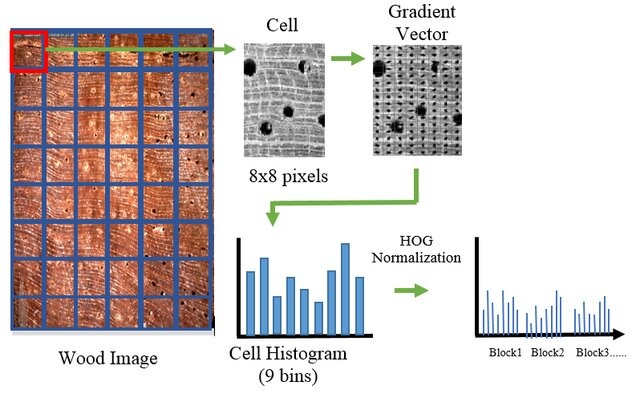
\includegraphics[width=1.0\textwidth]{images/hog_pipeline_visualization.jpg}
    \captionof{figure}{Quy trình tính toán đặc trưng HOG. (1) Vùng ảnh đầu vào. (2) Tính toán gradient. (3) Chia thành các ô $8 \times 8$. (4) Tính biểu đồ 9-bin cho mỗi ô. (5) Nhóm các ô $2 \times 2$ thành một khối và chuẩn hóa vector 36-D. (6) Lặp lại cho tất cả các khối chồng chéo để tạo vector HOG cuối cùng.}
    \label{fig:hog_pipeline}
\end{center}

\paragraph{Đánh giá thực nghiệm và bối cảnh:}
Theo kết quả trong nghiên cứu gốc của Dalal \& Triggs \cite{Dalal2005}, 
bộ mô tả HOG kết hợp với bộ phân loại tuyến tính SVM đạt độ chính xác phát hiện người đi bộ vượt trội so với các phương pháp dựa trên wavelet hoặc edge template thời đó. 
Trên bộ dữ liệu INRIA Person Dataset, HOG-SVM giảm sai số phát hiện xuống còn dưới 10\%, trong khi các phương pháp trước đó thường trên 40\%. 
Nhờ tính ổn định, tốc độ hợp lý và khả năng tổng quát cao, HOG đã trở thành nền tảng cho hàng loạt hệ thống nhận dạng và theo dõi đối tượng trong giai đoạn 2005–2012.

\subsubsection{Ứng dụng và So sánh}
\label{subsubsec:hog_applications}
\begin{itemize}
    \item \textbf{Ứng dụng chính:} HOG, kết hợp với một bộ phân loại tuyến tính như SVM, đã là phương pháp hàng đầu cho \textbf{phát hiện vật thể} trong nhiều năm, đặc biệt là phát hiện người đi bộ, xe cộ, và động vật.
    \item \textbf{So sánh với SIFT/SURF:}
        \begin{itemize}
            \item HOG là bộ mô tả \textbf{dày đặc} cho một vùng, trong khi SIFT/SURF là bộ mô tả \textbf{thưa thớt} cho các điểm.
            \item HOG được thiết kế để mô tả hình dạng toàn cục của một đối tượng trong một cửa sổ có kích thước cố định. SIFT/SURF được thiết kế để so khớp các điểm cục bộ riêng lẻ giữa các ảnh với tỷ lệ và góc nhìn khác nhau.
            \item HOG không có tính bất biến với xoay và tỷ lệ một cách tự nhiên (nó đòi hỏi phải tìm kiếm đối tượng ở nhiều tỷ lệ và góc độ khác nhau). SIFT/SURF được thiết kế để bất biến với các yếu tố này ngay từ đầu.
        \end{itemize}
\end{itemize}
Mặc dù HOG đã bị các phương pháp dựa trên CNN vượt qua về hiệu năng, các ý tưởng cốt lõi của nó—chia ảnh thành các ô, sử dụng biểu đồ hướng gradient, và chuẩn hóa cục bộ—vẫn còn nguyên giá trị và là nguồn cảm hứng cho nhiều kiến trúc mạng nơ-ron hiện đại.

\begin{table}[H]
	\centering
	\caption{So sánh giữa HOG và các bộ mô tả cục bộ (SIFT, SURF, ORB)}
	\begin{tabular}{lcccc}
		\toprule
		\textbf{Tiêu chí} & \textbf{HOG} & \textbf{SIFT} & \textbf{SURF} & \textbf{ORB} \\
		\midrule
		Mật độ đặc trưng & Dày đặc & Thưa & Thưa & Thưa \\
		Kích thước descriptor & Lớn (vài nghìn chiều) & 128 & 64 & 256 bit \\
		Bất biến xoay & Không (cần dò tìm đa góc) & Có & Có & Có \\
		Bất biến tỷ lệ & Không (cần dò tìm đa tỷ lệ) & Có & Có & Trung bình \\
		Tốc độ trích chọn & Nhanh & Trung bình & Nhanh & Rất nhanh \\
		Ứng dụng chính & Phát hiện vật thể & So khớp đặc trưng & So khớp/3D & SLAM/AR \\
		Miễn phí bản quyền & Có & Không & Không & Có \\
		\bottomrule
	\end{tabular}
\end{table}

\subsection{Tổng kết: Ưu, nhược điểm và Di sản của Đặc trưng Thủ công}
\label{subsec:handcrafted_pros_cons}

Các bộ phát hiện và mô tả đặc trưng thủ công như SIFT, SURF, ORB, và HOG đã thống trị lĩnh vực Thị giác Máy tính trong gần hai thập kỷ. Chúng là những thành tựu kỹ thuật đáng kinh ngạc, đặt nền móng cho vô số ứng dụng và định hình nên tư duy của cả một thế hệ nhà nghiên cứu. Việc phân tích ưu và nhược điểm của chúng không chỉ là một bài tập lịch sử, mà còn giúp chúng ta hiểu rõ hơn những vấn đề mà học sâu đã giải quyết và những thách thức vẫn còn tồn tại.

\subsubsection{Ưu điểm: Sự Minh bạch, Hiệu quả và Nền tảng Lý thuyết Vững chắc}
\label{subsubsubsec:handcrafted_pros}
\begin{description}
    \item[Tính Minh bạch và Khả năng Diễn giải (Transparency \& Interpretability):] Đây là ưu điểm lớn nhất của các phương pháp cổ điển so với các mô hình học sâu "hộp đen". Mỗi bước trong thuật toán SIFT hay HOG đều được thiết kế dựa trên một nguyên lý toán học hoặc một trực giác rõ ràng về xử lý tín hiệu. Khi một thuật toán so khớp SIFT thất bại, chúng ta có thể đi sâu vào từng bước để phân tích nguyên nhân.
    
    \item[Hiệu quả Dữ liệu (Data Efficiency):] Các thuật toán này không đòi hỏi quá trình "huấn luyện" trên một tập dữ liệu khổng lồ có gán nhãn. Chúng được xây dựng dựa trên các nguyên lý toán học phổ quát và có thể hoạt động "ngay lập tức" trên một hình ảnh mới.
    
    \item[Hiệu suất Tính toán Có thể Dự đoán (Predictable Computational Performance):] Các thuật toán như FAST và ORB được thiết kế đặc biệt để có tốc độ cực cao trên CPU, một yêu cầu quan trọng cho nhiều ứng dụng nhúng.
    
    \item[Nền tảng Lý thuyết Vững chắc:] Việc phát triển các đặc trưng thủ công đã thúc đẩy nhiều nghiên cứu nền tảng quan trọng về hình học chiếu, không gian tỷ lệ, và xử lý tín hiệu.
\end{description}

\subsubsection{Nhược điểm: Sự Mong manh và Giới hạn của Chuyên môn Con người}
\label{subsubsubsec:handcrafted_cons}
Chính những hạn chế của đặc trưng thủ công đã tạo ra nhu cầu cấp thiết cho một cuộc cách mạng, và học sâu đã đáp ứng lời kêu gọi đó.

\begin{description}
    \item[Sự Mong manh (Brittleness) trước các Biến đổi Phức tạp:] Mặc dù các thuật toán như SIFT được thiết kế để bất biến với một số loại biến đổi nhất định, chúng vẫn rất "mong manh" khi đối mặt với sự đa dạng của thế giới thực như biến dạng phi tuyến, thay đổi ánh sáng phức tạp (bóng đổ, phản xạ), và sự che khuất (occlusion).
    
    \item[Tính Tổng quát Kém (Poor Generalization):] Các đặc trưng thủ công được thiết kế dựa trên các giả định về các loại cấu trúc tồn tại trong ảnh (ví dụ: các cạnh sắc nét, các góc). Chúng hoạt động tốt trên các vật thể nhân tạo, có kết cấu, nhưng lại hoạt động rất kém trên các bề mặt không có kết cấu, các vật thể có thể biến dạng (quần áo), hoặc các loại hình ảnh chuyên biệt (ảnh y khoa).
    
    \item[Giới hạn bởi Chuyên môn của Con người:] Hiệu suất của toàn bộ hệ thống bị giới hạn bởi sự thông minh của người thiết kế ra bộ trích xuất đặc trưng. Con người chỉ có thể mã hóa những gì chúng ta có thể mô tả một cách hình thức. Có vô số các mẫu và kết cấu tinh vi trong thế giới tự nhiên mà chúng ta không thể định nghĩa bằng một vài dòng mã lệnh. Đây là "nút thắt cổ chai" lớn nhất của kỷ nguyên cổ điển.
    
    \item[Quy trình Nhiều bước Rời rạc:] Một pipeline cổ điển bao gồm nhiều bước (phát hiện, mô tả, so khớp) được thiết kế và tối ưu hóa một cách độc lập. Điều này có thể dẫn đến việc các sai số từ các bước đầu sẽ tích tụ và lan truyền, và toàn bộ hệ thống không được tối ưu hóa một cách end-to-end cho tác vụ cuối cùng.
\end{description}

\subsubsection{Cầu nối sang Học sâu}
\label{subsubsubsec:handcrafted_bridge_to_dl}
Tóm lại, kỷ nguyên của các đặc trưng thủ công đã dạy cho chúng ta những bài học vô giá về việc \textit{phải tìm kiếm những gì} trong một bức ảnh: các cấu trúc đa tỷ lệ, các phân bố gradient cục bộ, và sự cần thiết của tính bất biến. Nhưng nó cũng cho thấy rằng việc "thiết kế" các quy tắc một cách thủ công là một con đường có giới hạn.

Câu hỏi tự nhiên tiếp theo là: Thay vì để các chuyên gia con người thiết kế các bộ lọc và quy tắc này, liệu chúng ta có thể để cho máy tính \textbf{tự học} các đặc trưng tốt nhất trực tiếp từ dữ liệu không? Liệu có thể xây dựng một hệ thống được tối ưu hóa end-to-end, từ pixel đầu vào đến quyết định cuối cùng? Câu trả lời là "Có", và đó chính là lời hứa của Học sâu và Mạng nơ-ron Tích chập (CNN), chủ đề mà chúng ta sẽ khám phá trong chương tiếp theo.

\section*{Tài liệu tham khảo}
\begin{itemize}
    \item[1] Lowe, D. G. (2004). Distinctive Image Features from Scale-Invariant Keypoints. \textit{International Journal of Computer Vision}, \textit{60}(2), 91–110.
    \item[2] Bay, H., Ess, A., Tuytelaars, T., \& Van Gool, L. (2008). Speeded-Up Robust Features (SURF). \textit{Computer Vision and Image Understanding}, \textit{110}(3), 346–359.
    \item[3] Rublee, E., Rabaud, V., Konolige, K., \& Bradski, G. (2011). ORB: An efficient alternative to SIFT or SURF. In \textit{Proceedings of the International Conference on Computer Vision (ICCV)}.
    \item[4] Dalal, N., \& Triggs, B. (2005). Histograms of Oriented Gradients for Human Detection. In \textit{Proceedings of the IEEE Conference on Computer Vision and Pattern Recognition (CVPR)}.
    \item[5] Calonder, M., Lepetit, V., Strecha, C., \& Fua, P. (2010). BRIEF: Binary Robust Independent Elementary Features. In \textit{European Conference on Computer Vision (ECCV)}.
    \item[6] Rosten, E., \& Drummond, T. (2006). Machine learning for high-speed corner detection. In \textit{European Conference on Computer Vision (ECCV)}.
\end{itemize}